\documentclass[10pt, a4paper]{article}
\usepackage[top=0.6in,bottom=1.0in,left=1.0in,right=1.0in]{geometry}
\usepackage{amsmath,amssymb}
\usepackage{graphicx,float,tikz}
\usepackage{listings}

\fontfamily{times}
\usepackage[colorlinks = true,
            linkcolor = black,
            urlcolor  = blue,
            citecolor = blue,
            anchorcolor = blue]{hyperref}

\begin{document}
\begin{titlepage}
	\begin{center}
		\begin{Large}
		
		\vspace*{4cm}
		\centerline{ 	
 			
\includegraphics[scale=.9]{logo.png}
		}
		\textbf{CS 4366: Senior Capstone Project \\ Dr. Sunho Lim \\ Texas Tech University \\ Project \#5 \\ Validation and Full Demo \\ EmergenSeek}
 
		\vspace{0.5cm}
		Spring 2019 Final Report 
		\linebreak
 		by \\
		\textbf{Suhas Bacchu \\ Derek Fritz \\ Kevon Manahan \\ Annie Vo \\ Simon Woldemichael}
 
		\newpage
 		\end{Large}
	\end{center}
\end{titlepage}

\vspace*{\fill}
\begin{abstract}
In this final report, we describe and detail the validation of EmergenSeek, a multiuse, cross-platform mobile application providing simple access to emergency services and contact connections. As with previous reports, we will structure the report by enumerating on the frontend and backend. Dissimilarly, we will only describe necessary details in the validation of our implementations, to the extent that, any other developer with some programming background will be able to successfully implement our system's components. Only necessary details will be presented to the reader and care should be taken when reading them\footnote{Concepts such as continuous integration, continuous deployment, microservices, serverless computing, NoSQL databases, APIs, and widget-based mobile development will be discussed. These new concepts may be difficult to grasp initially, but sufficient details will be provided.}. Restatements from previous deliverable reports will be made to remind the reader of pre-defined, but important information. Also, a glossary is provided at the end of the report to define terms and jargon that may be confusing or unfamiliar for the reader. \\
\textit{Keywords:} API Gateway, CI/CD, Cloud, Dart, Flutter, Golang, Lambda, Mobile, Serverless
\end{abstract}
\vspace*{\fill}
\newpage

\tableofcontents
\newpage


\section{Introduction}
\par ~ The development of EmergenSeek has been an effective software engineering experience for our group. In this final submission, we will discuss our project by first restating the idea, project motivations, and our successful implementations. Then, we will discuss the final state of our UML diagrams and architecture, for this Spring semester. After, we will discuss the development cycle for the frontend and backend and briefly touch on the microservices architecture that we follow. 

\par ~ Next, a walkthrough of the discussed development lifecycle, using only necessary details and supplementing those details with additional code comments, snippets, and screenshots. This walkthrough will allow the user to understand the structure of our application, both frontend and backend. The walkthrough will not cover \emph{everything} as the amount of content necessary for a walkthrough that assumes the reader has zero prior knowledge of the systems and concepts used in our project would take an obstructive amount of explanation. Then, we will describe the current state of our serverless application repository; our collection of Lambda functions. To end on our discussion of the validation, we will display Flutter views of the mobile application and their respective functionality. 

\par ~ It is very important to note that our project uses programming languages which are young in maturity and may not be familiar to the reader. But, our backend, written in Go, has syntax very similar to the C and C++ programming languages. Our frontend, written in Dart, has syntax very similar to the Java programming language. As a result of these similarities, it is permissible for the reader to assume what the code does as the syntax is, for the most part, straightforward. To conclude we will detail team member contributions, implementation issues, and steps moving forward with the project.

\subsection{Walkthrough Steps}
\par ~ The previously mentioned walkthrough will consist of the following, and be enumerated for a single Lambda function and a single Flutter application screen. This section should be referred to in the \hyperref[sec:pdl]{Project Development Lifecycle} section:
\begin{enumerate}
	\item[1.] Feature expectation. Answer the question of ``What feature do we need to implement and how do we implement it?''
	\item[2.] Lambda function: Implement the feature and its expectations around the requirements of using AWS Lambda
	\item[3.] Informal testing: Get an initial working version of the API Lambda function
	\item[4.] Formal testing: Write unit tests for the implementation
	\item[5.] Integration and Infrastructure as Code: Define the deployment
	\item[6.] Continuous Integration: Do the deployment
	\item[7.] Integrate Lambda functionality with the frontend
	\begin{itemize}
		\item[7a.] Create feature view. The view is effectively the screen that the user will interact with.
		\item[7b.] Create feature model. Define how features will be referenced by the state of the application.
		\item[7c.] Interface with Lambda function. Make calls via an HTTP client to the Lambda function
	\end{itemize}
\end{enumerate}

\par ~ As all of our project code is open-source, readers are encouraged to reference the code repositories for our project. They are located at \url{https://github.com/emergenseek/backend} and \url{https://github.com/emergenseek/Flutter-Client} for our backend and frontend code, respectively. Readers who would like more insight, or have questions are welcome to open an issue or pull request on either of these GitHub repositories.

\section{Project Overview}
\subsection{Project Definition, and Implemented Features}
\par ~ EmergenSeek is a mobile application which provides users with multiuse, centralized emergency information and notification services. This application gives friends and family members priority connections in times of emergency or crisis. Our sucessfully implemented, core feature are as follows:

\begin{enumerate}
	\item[1.] S.O.S. button emergency broadcast --- Users are able to utilize the mobile client to invoke an S.O.S. button for automated notification of contacts and emergency services. 
	\item[2.] Emergency service locator --- Users are able to utilize the mobile client to search for emergency service (hospitals, and pharmacies). Currently, searching will return results up to a fixed radius of 20 miles.
	\item[3.] Granular permission definitions for contacts --- The user is given full control over what contacts receive what level of information. This is achieved by setting alert tiers on a per-contact basis.
	\item[4.] Lock screen display of health information for emergency services --- In the case of an S.O.S. situation, the user shall have their health information displayed for the convince of first respondents.
\end{enumerate}

\par ~ Additionally, successfully implemented, quality of user-experience features are as follows. While the application is still functional without them, deploying the application for public, functional use, cannot not be possible without them.
\begin{enumerate}
	\item[1.] User registration and login --- Users are able to register for an account and track their personal information, necessary in an emergency event.
	\item[2.] Settings persistence -- Users are able to change settings within the application to fit their preference.
\end{enumerate}

\subsection{Features In-progress}
\par ~ Features which are partially implemented are as follows:
\begin{enumerate}
	\item[1.] Periodic notifications to contacts (location-based polling) --- The user shall be able to utilize the mobile client to send periodically send their location information to contacts. While the logic is in-place, we currently do not have a successful implementation of repeating the location polling.
	\item[2.] Retrieval of international emergency service numbers (ambulance, fire, and police), depending on the user's current location. Connections to the front-end have not been made yet.
\end{enumerate}

\subsection{Future Features}
\par ~ Lastly, additional quality of user-experience features that have not been, but maybe implemented in the future are:
\begin{enumerate}
	\item[1.] More extensive error handling and reporting (via something like the Catcher, a Flutter package or Sentry.io a multi-language, multi-framework error reporting and management service)
	\item[2.] More in-depth user preferences, settings and options
	\item[3.] Alternative sign-up and log-in methods (Google, Facebook, etc.)
\end{enumerate}

\section{UML and Design Documentation}
\par ~ In this section we will discuss our completed Unified Modeling Language (UML) diagrams and design documents. Items are presented with a figure of the design unit and briefly described.

\subsection{Use-case Diagram}

\begin{figure}[H]
\begin{center}
\centerline{
	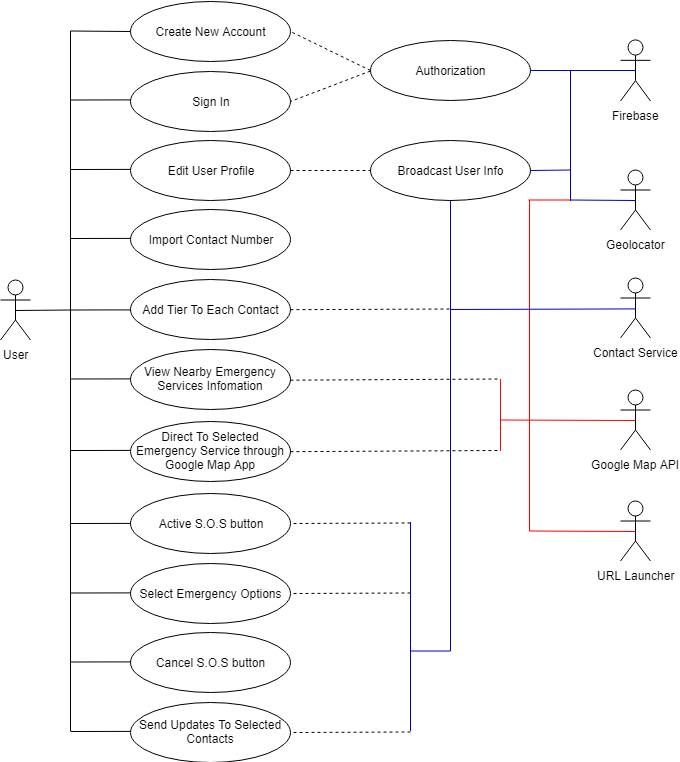
\includegraphics[scale=.6]{final-diagrams/Revised_Use_Case_Diagram.png}
}
\caption{Updated use-case diagram for the EmergenSeek application.}
\end{center}	
\end{figure}
\par ~ In this use-case diagram we detail external dependencies and their inclusion to each of the use cases. Authorization is dependent on Google's Firebase service. The broadcasting of user info is depending on using MapQuest's Geolocator API. The contact service allows us to read contacts directly from the user's phone. It is important to note that this has only been tested on Android devices. The Google Maps API coupled with the URL launcher allows us to connect our service locator with the user's native Google Maps application. Whenever the user selects a location, they will be directed to the location by tapping on the marker associated with it. Creating new accounts and signing the user in extend the authorization item. All S.O.S. button and emergency related use-cases extend the broadcasting of user info to the backend. 


\subsection{Class Diagrams}
\subsubsection{Frontend}
\par ~ For frontend class diagrams, we will first show the full models, then discuss the models, broken up into 3 smaller components, Views, Models, and Services. 
\begin{figure}[H]
\begin{center}
\centerline{
	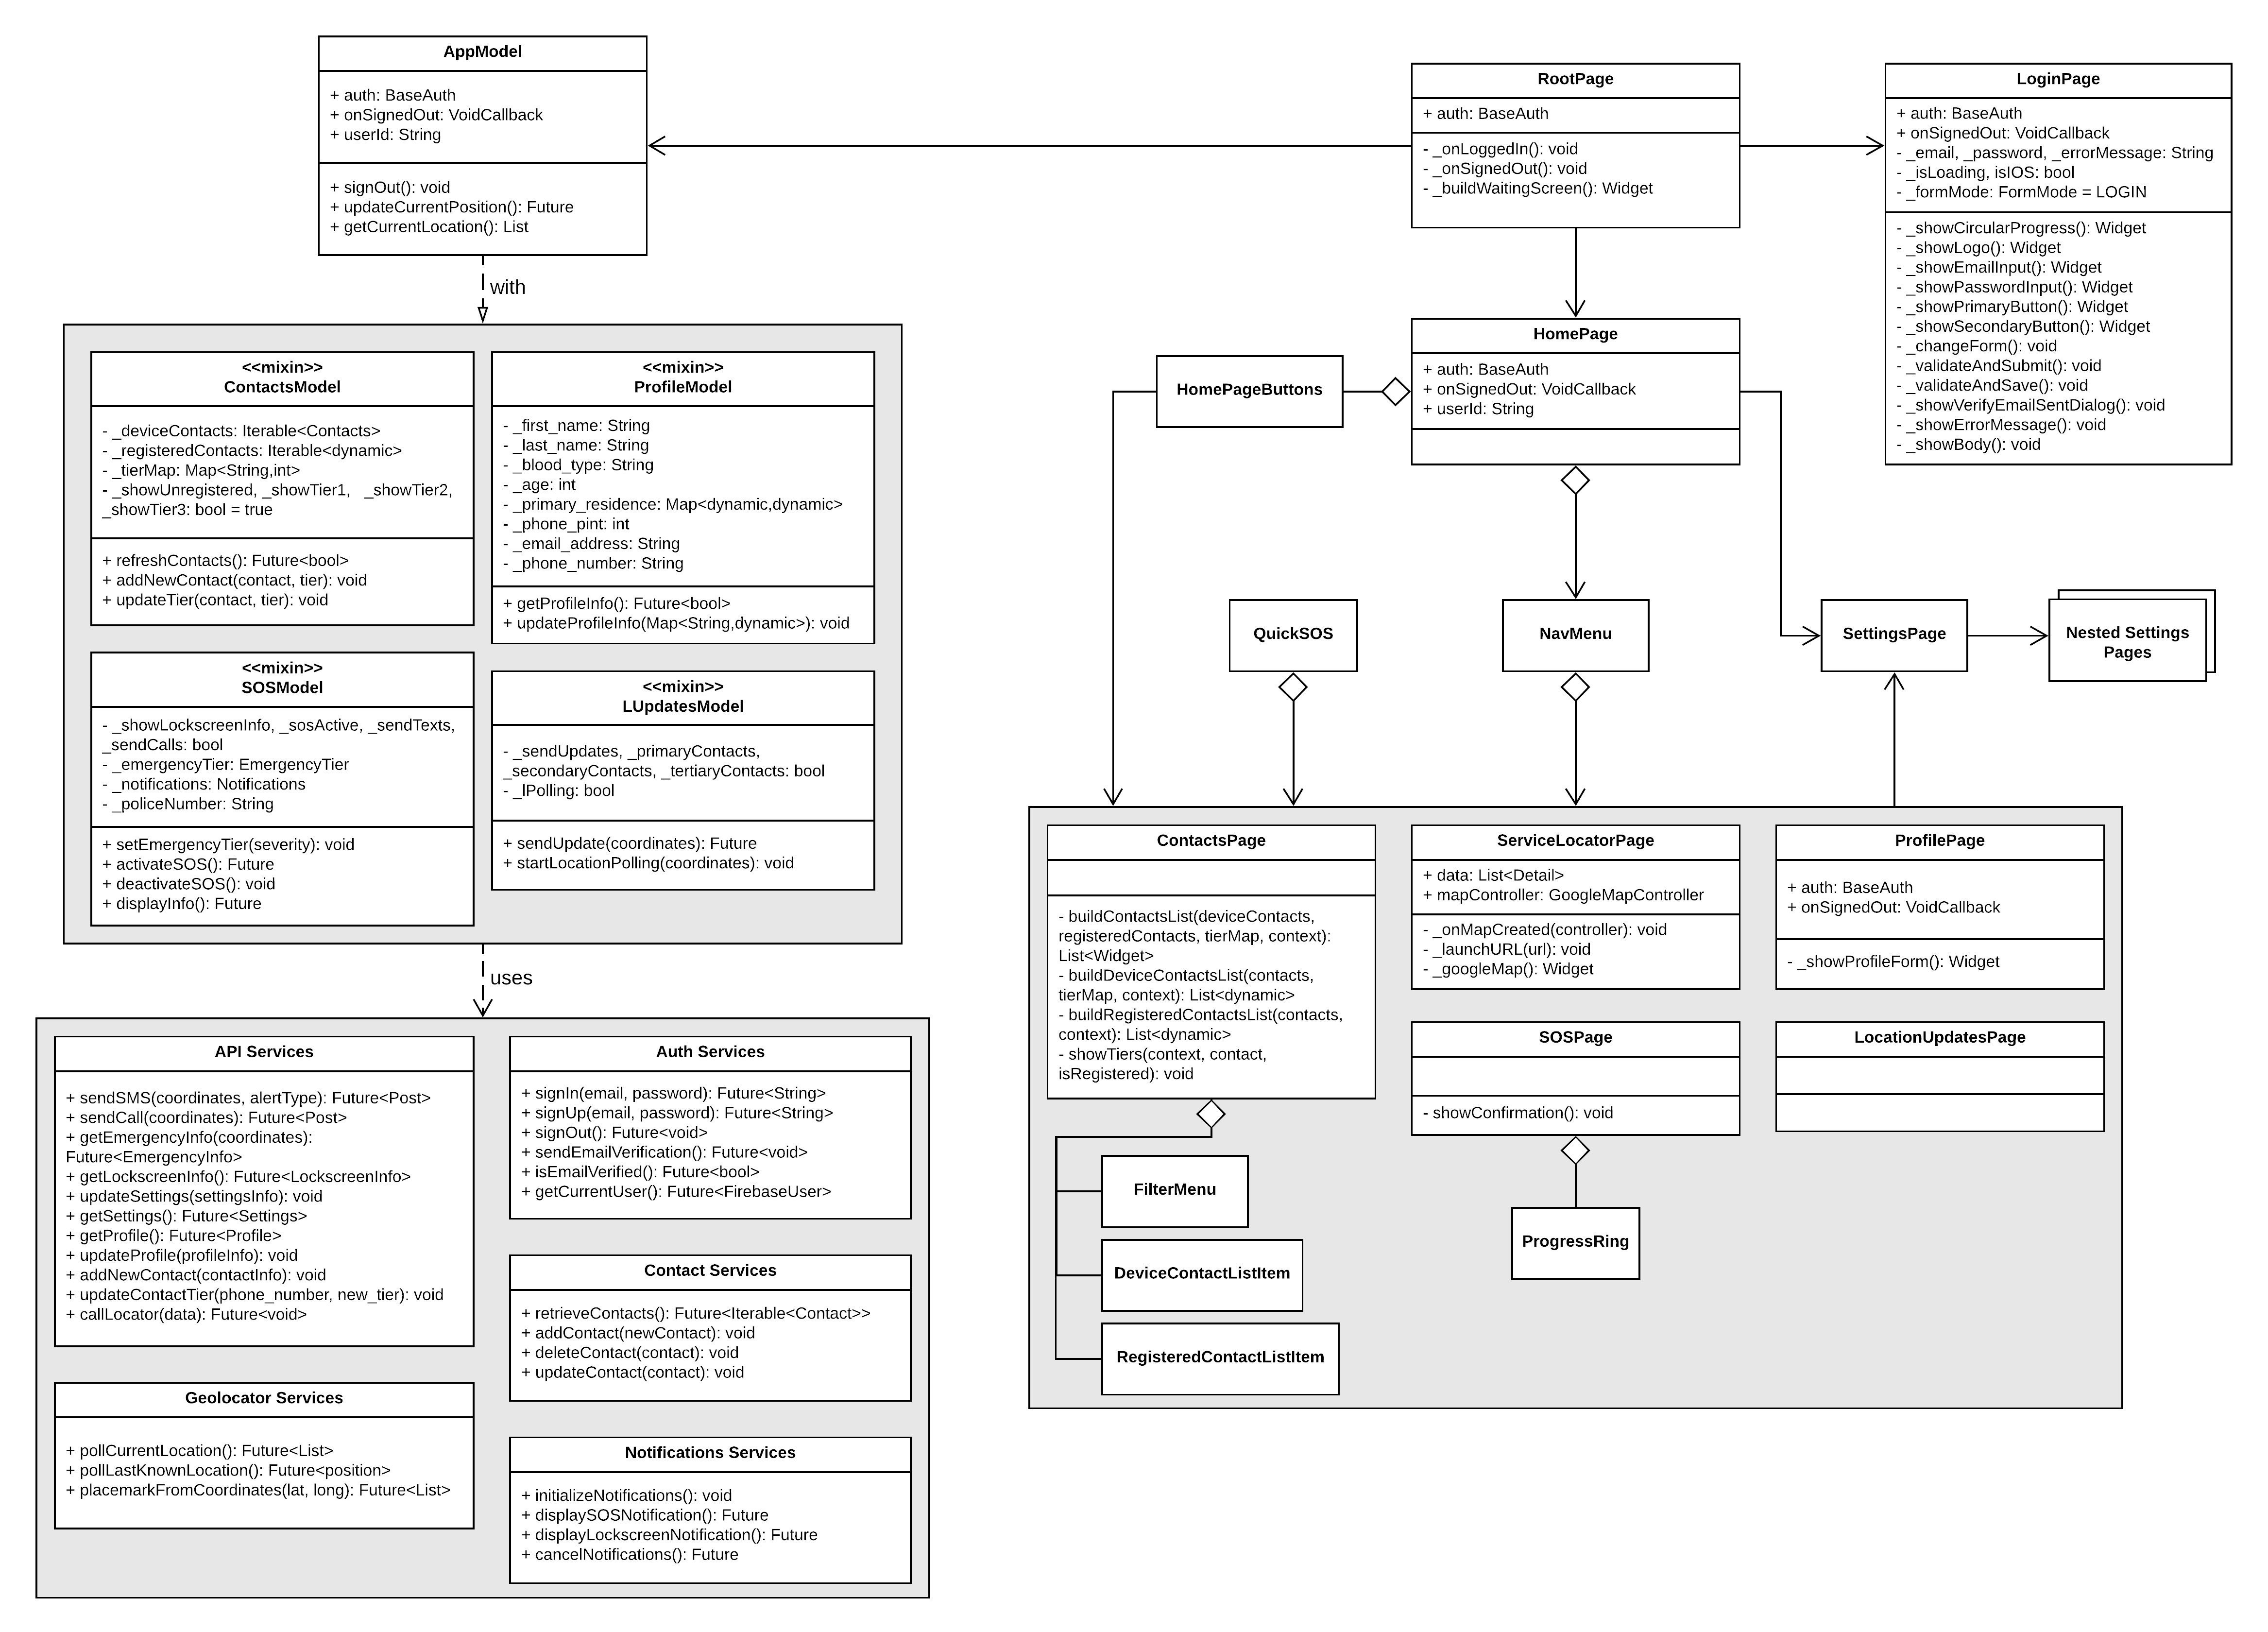
\includegraphics[scale=.13]{final-diagrams/EmergenSeek-Class-Diagram.png}
}
\caption{Full class diagram for the frontend.}
\end{center}	
\end{figure}

\begin{figure}[H]
\begin{center}
\centerline{
	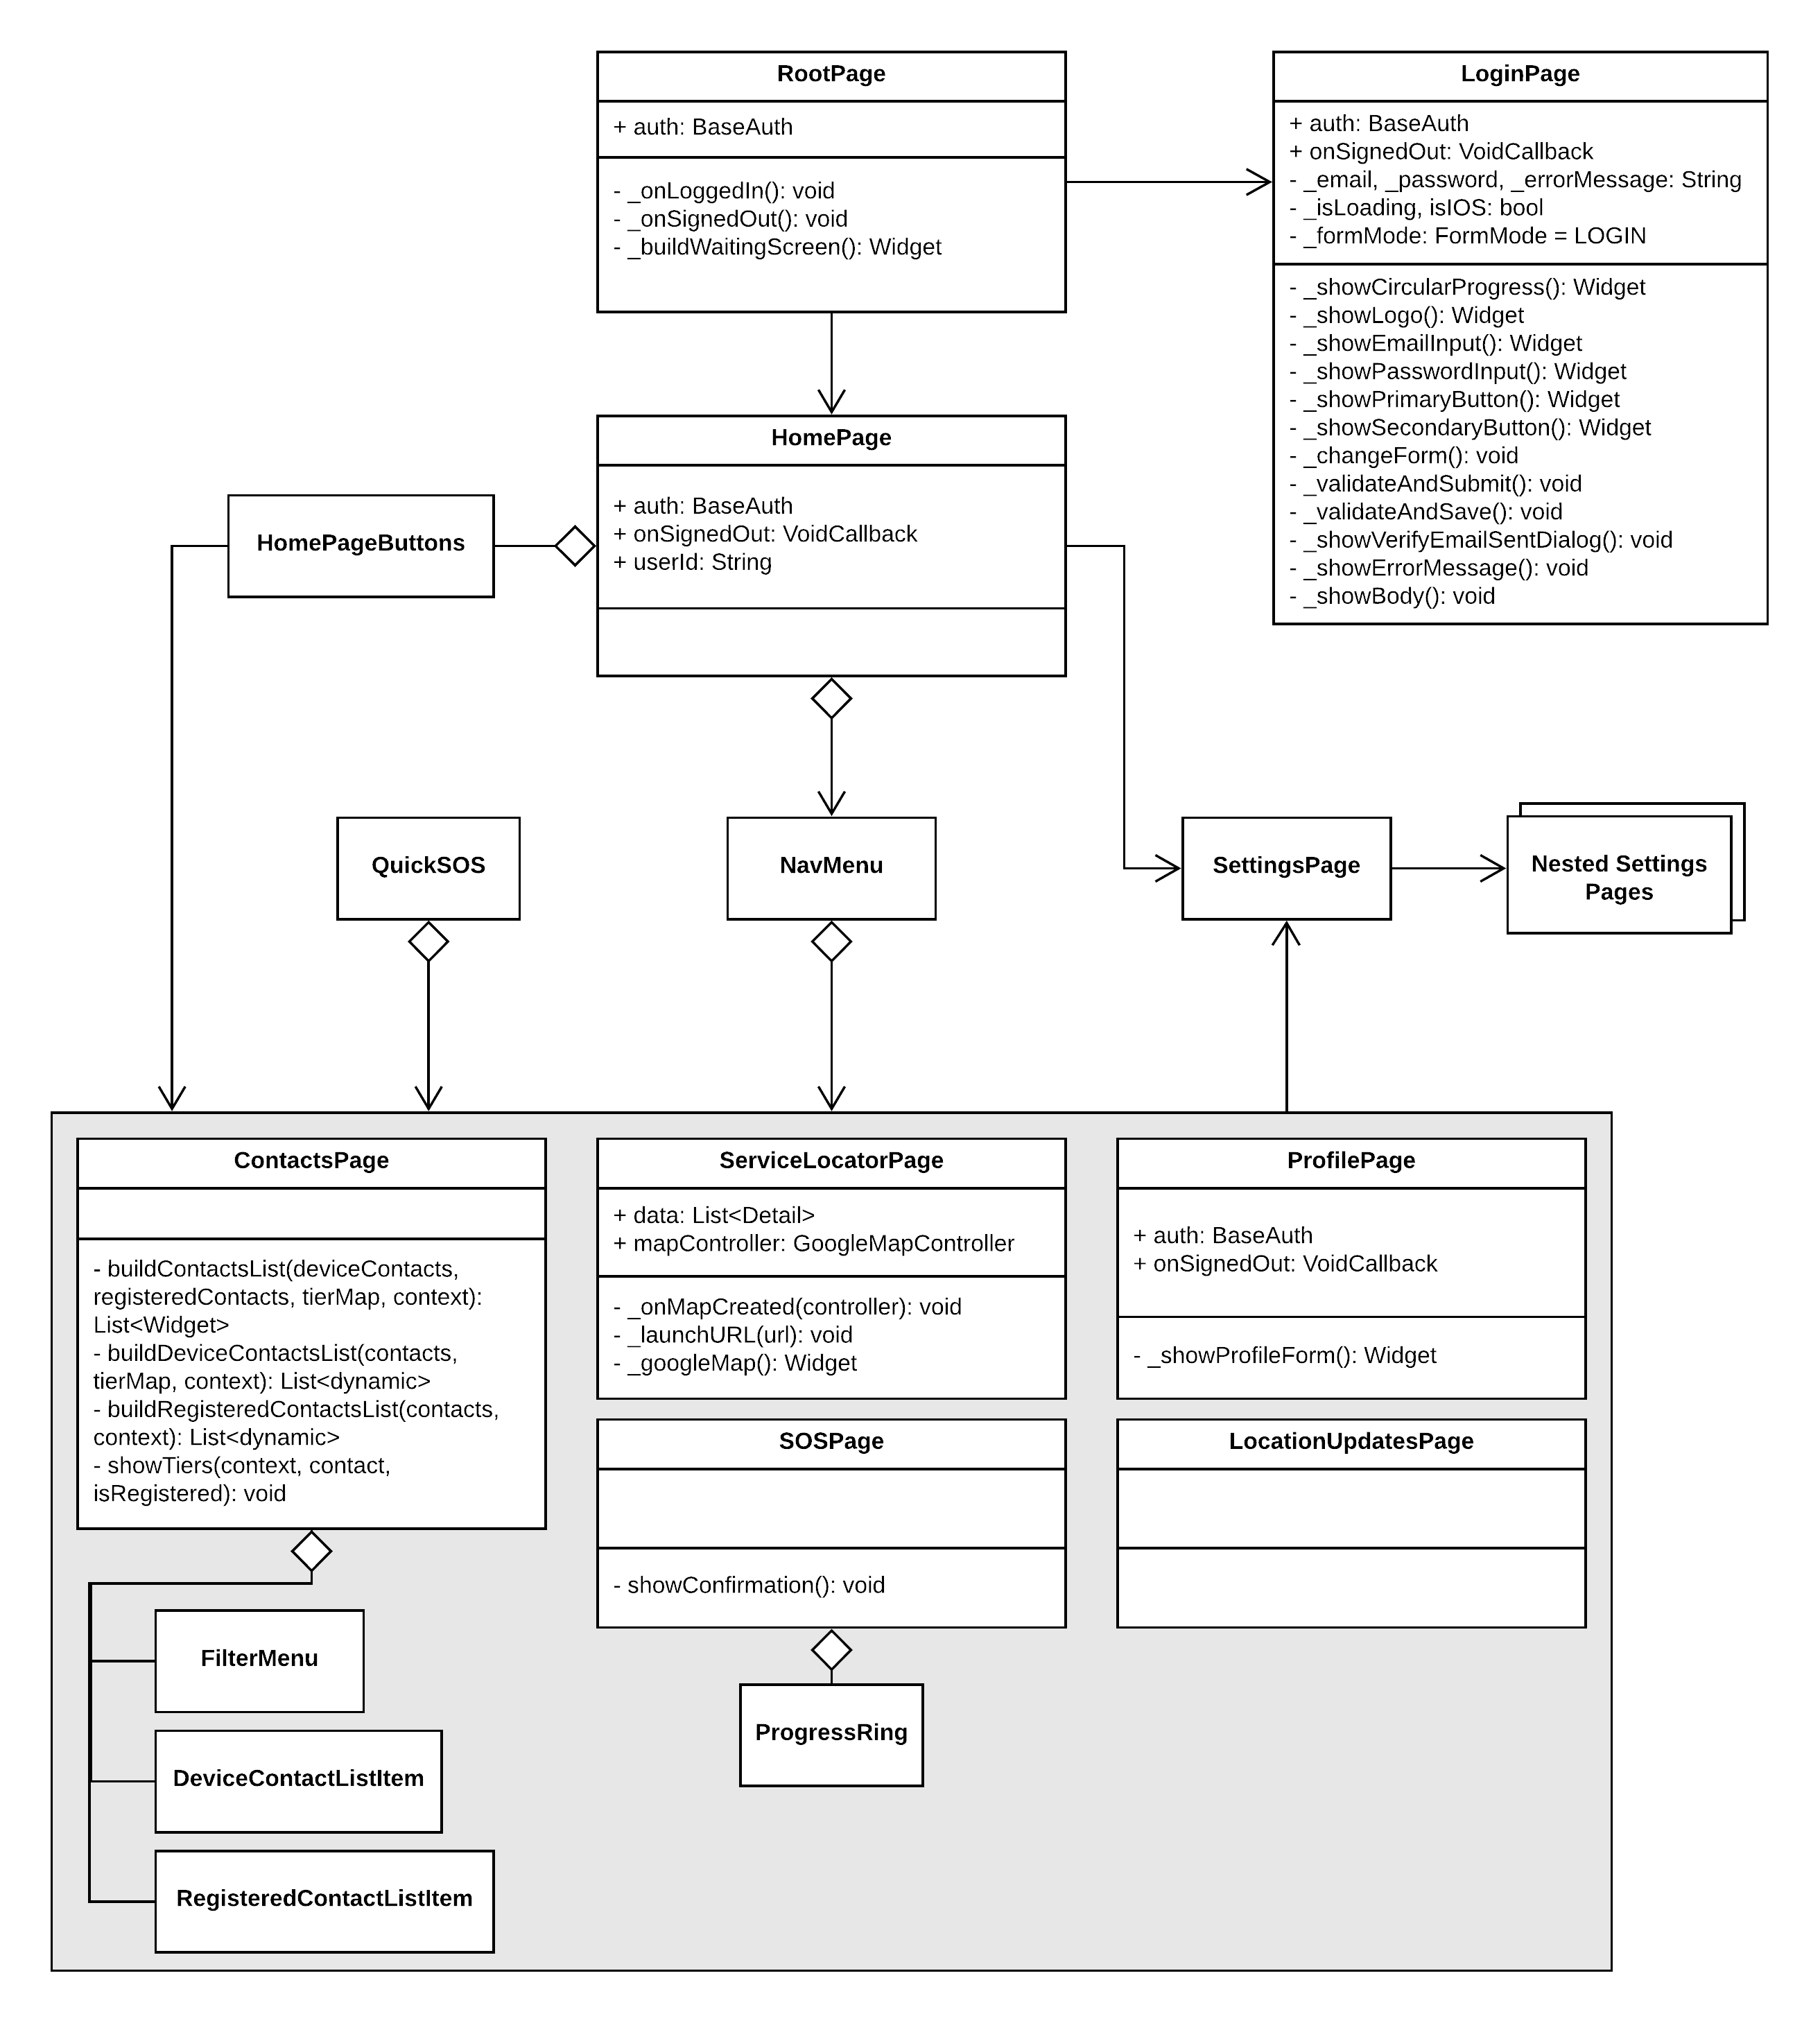
\includegraphics[scale=.23]{final-diagrams/Views-UML.png}
}
\caption{View UML class diagram for the frontend.}
\end{center}	
\end{figure}

\par ~ The application's views begins via a RootPage, this root page can be thought of a session manager keeping track of the user though an \texttt{auth} object. This object tracks actions that occur on certain events; if the user is logged in, signed out, or waiting for some communication with the backend to complete. This session state is managed via the LoginPage. From the RootPage we have a HomePage. This homepage is displayed once the base authentication, encapsulated as an attribute of the RootPage class, has received a successful response from Firebase and tells the application that the user is authorized. From the home page, we have buttons that connect the user to other views. These views, ContactsPage, ServiceLocatorPage, PorfilePage, LocationUpdatesPage, menus and navigations are displayed at the end of our report. 

\begin{figure}[H]
\begin{center}
\centerline{
	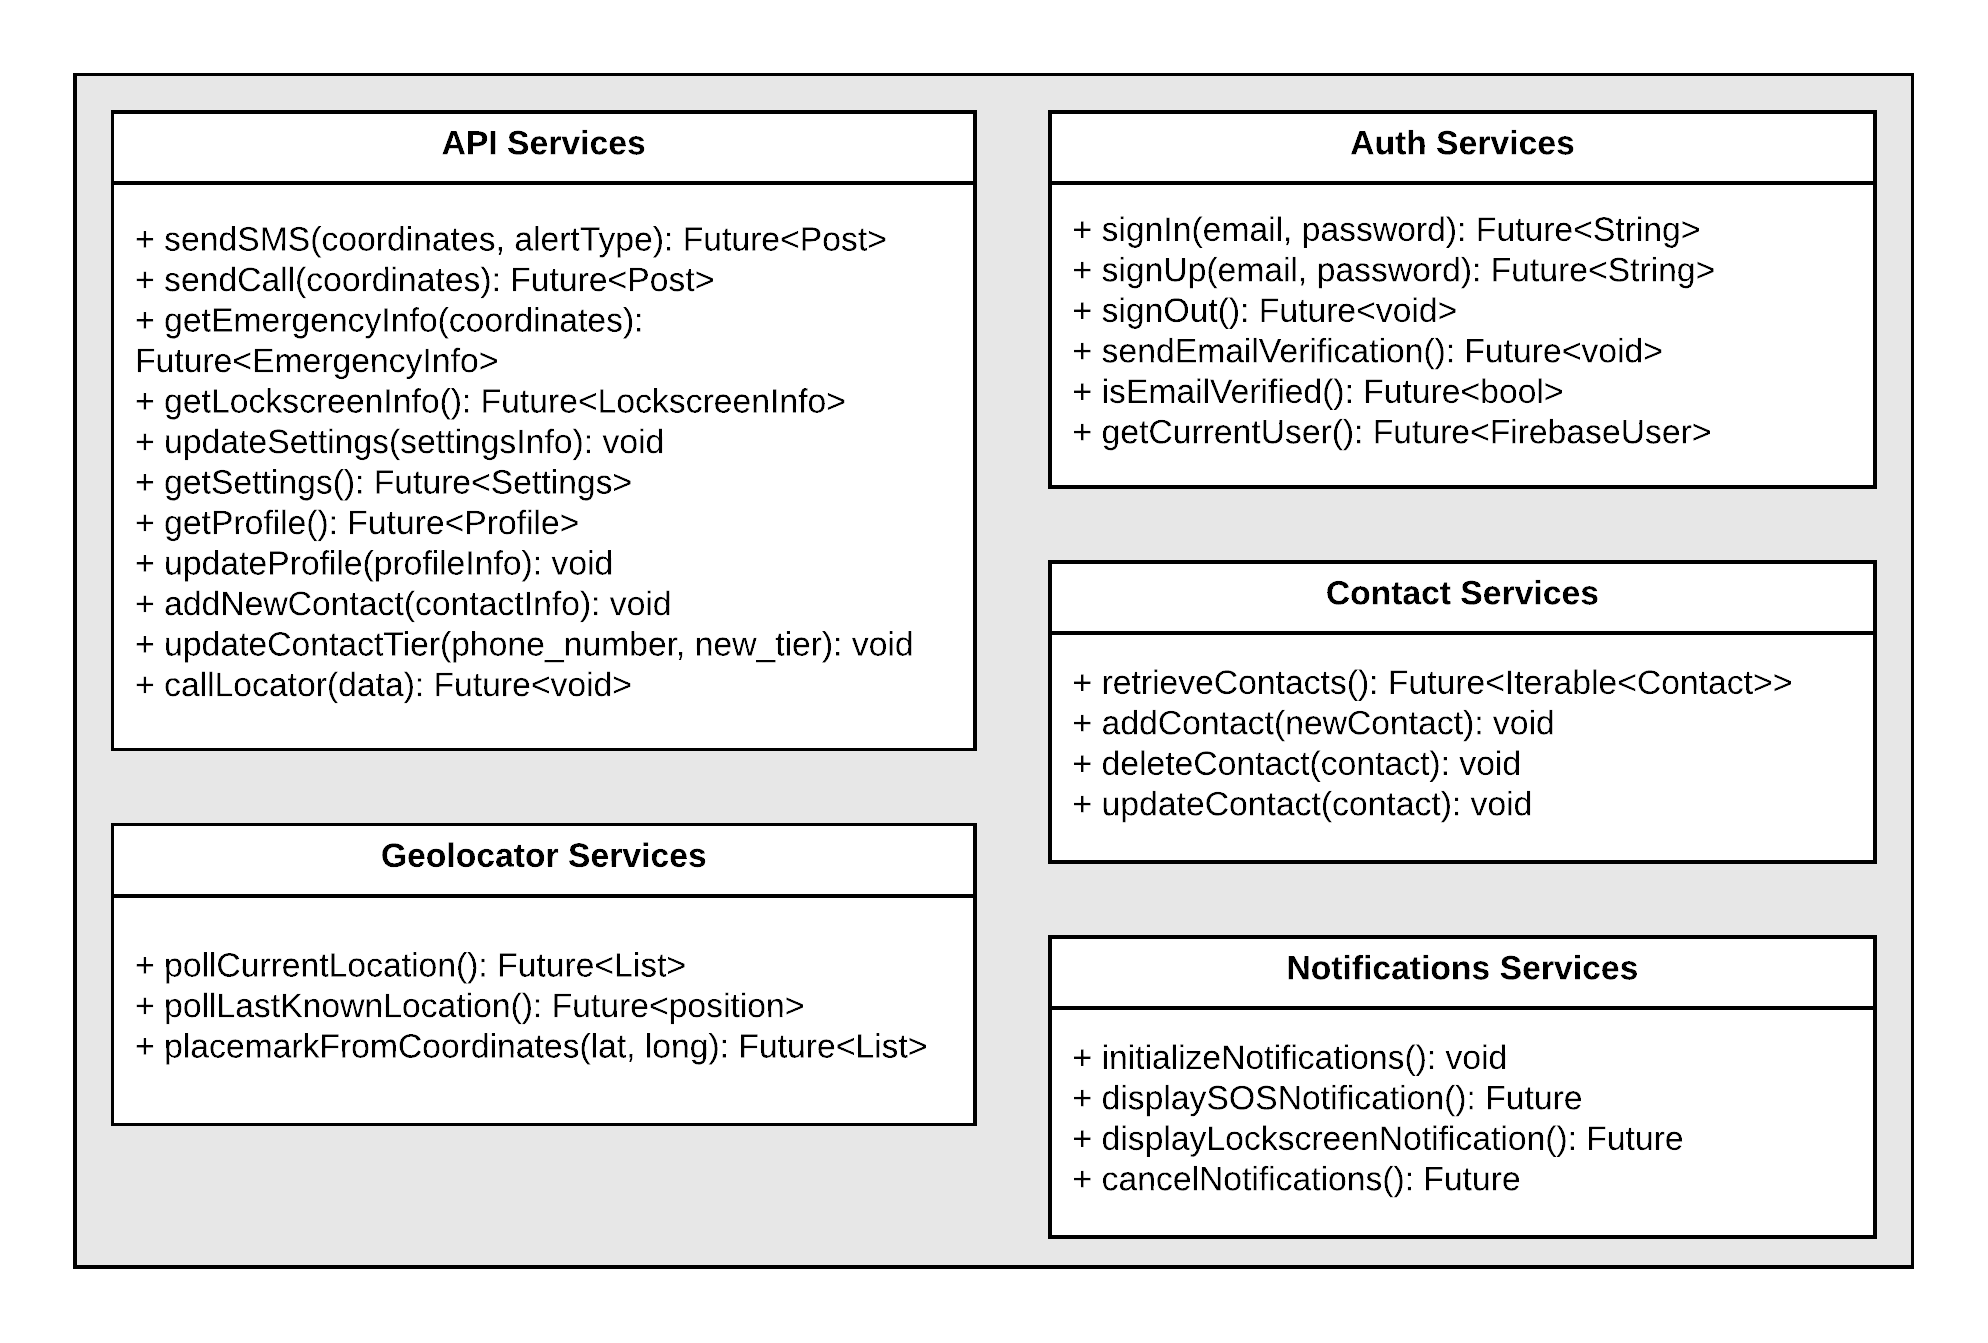
\includegraphics[scale=.23]{final-diagrams/Services-UML.png}
}
\caption{Service UML class diagram for the frontend.}
\end{center}	
\end{figure}

\par ~ The application's services are necessary for managing external API's, both Firebase and our Lambda functions. The API services class encapsulates many, general API endpoints proxied by AWS API Gateway. The Auth Services clas communicates with Firebase to register, login, and logout users. The Geolocator Services class entails methods necessary for the Google Maps integrate map we use for our service locator. The Contact Services class communicates with the native contacts API on the device's host operating system to retrieve the user's contacts. The Notifications Services class encapsulate methods necessary for displaying notifcations on the device, both within the notifications center and on the user's lock screen. \\

\begin{figure}[H]
\begin{center}
\centerline{
	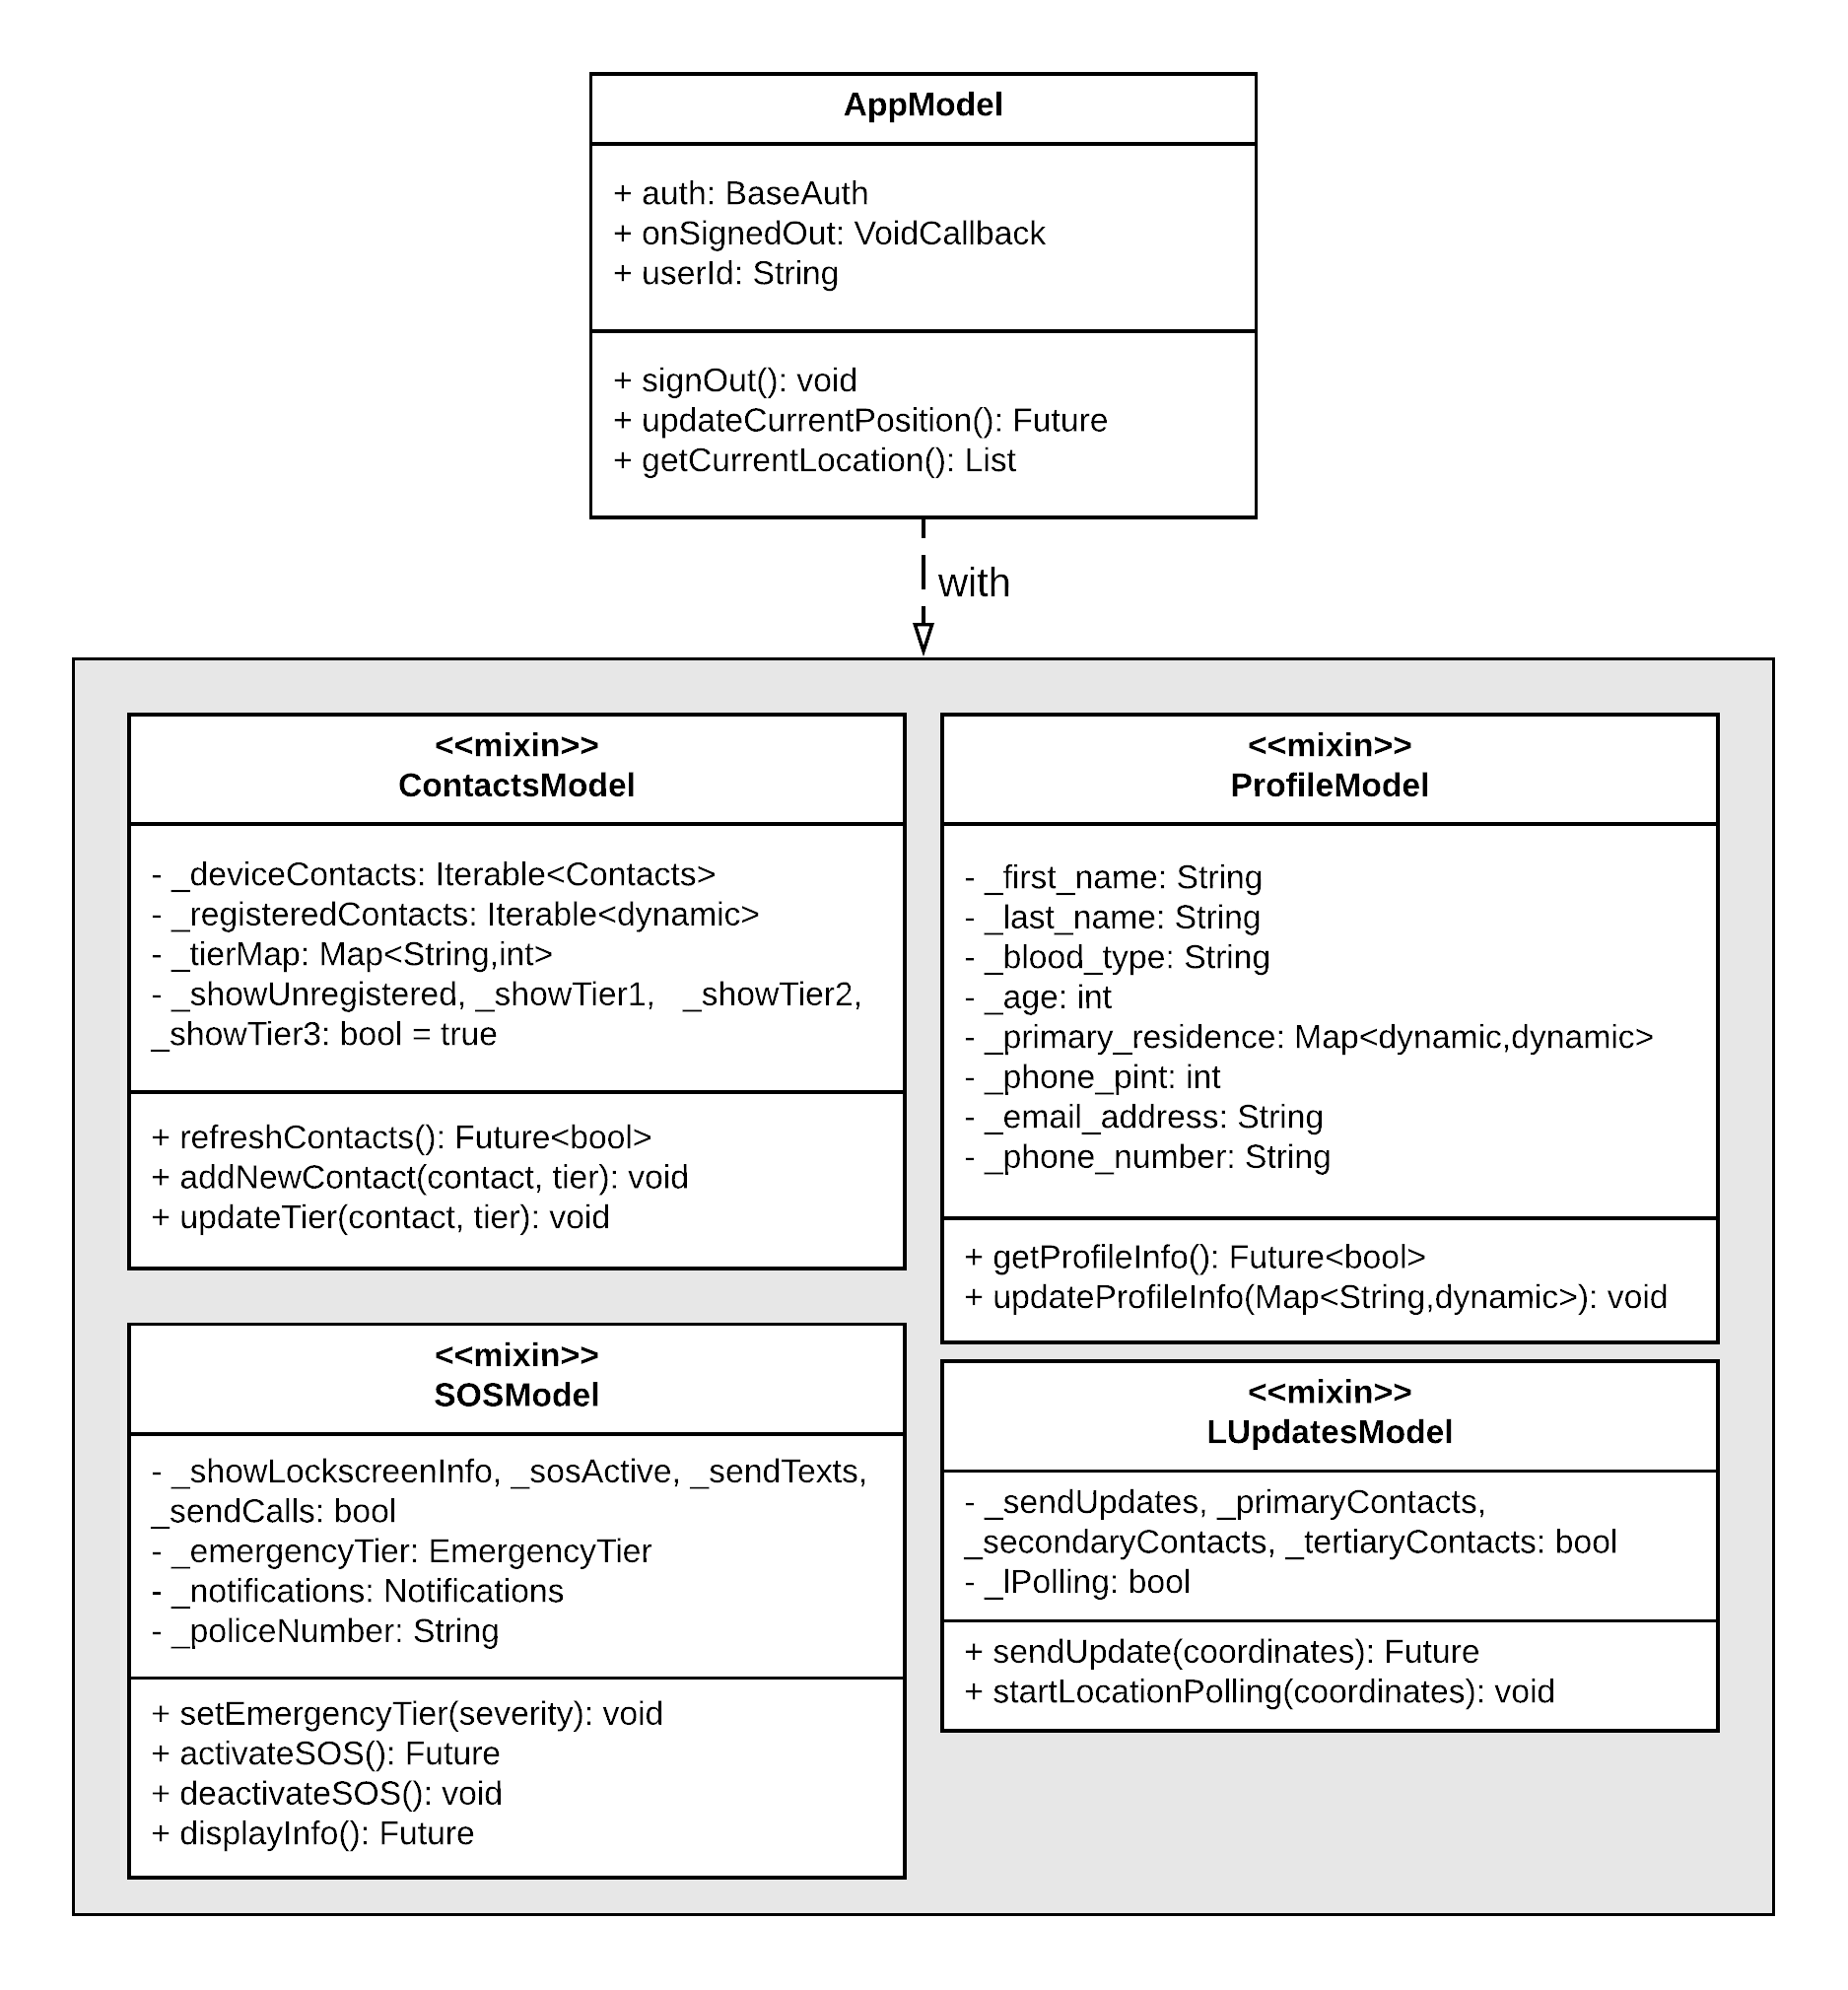
\includegraphics[scale=.37]{final-diagrams/Models-UML.png}
}
\caption{Model UML class diagram for the frontend.}
\end{center}	
\end{figure}

\par ~ The application's models and global state are tracked in an AppModel instance, this AppModel is how variables and application flow is tracked, regardless of what view the user is interacting with. The AppModel then has several \texttt{mixin} objects. A mixin, similar to inheritance, is a class which requires functionality from other base classes, but does not need to become the parent of that class. Though mixins, multiple inheritance is possible and allows our application to utilize the scoped models, discussed below.

\subsubsection{Backend}
\begin{figure}[H]
\begin{center}
\centerline{
	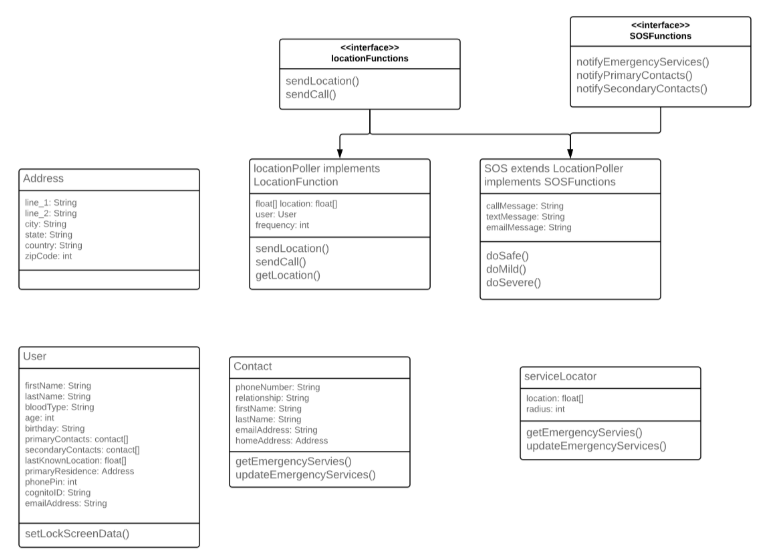
\includegraphics[scale=1]{final-diagrams/backend-class.PNG}
}
\caption{Class diagram for the EmergenSeek backend.}
\end{center}	
\end{figure}

\par ~ No major changes have been made to this document since previous report previsions. This class diagram should be used as a loose reference and not a literal representation of how our backend is structured for reasons related to how Go programs are written. In this class diagram for our backend we have:
\begin{enumerate}
	\item[1.] Address --- Encapsulates the data necessary for representing an address.
	\item[2.] User --- Encapsulates the data necessary for representing a user. Has 1 method which retrieves the user's information using a Lambda function for display on the lock screen.
	\item[3.] Contact --- Encapsulates the data necessary for representing a user's contact. Has 2 methods which get and update the contact on the emergency services map so that the user may see which of their contacts are nearby.
	\item[4.] ServiceLocator --- Encapsulates the data necessary for performing location based functions. Has two methods which will get and update emergency service locations for the map on the client.
	\item[5] LocationFunctions --- (Interface) This interface contains the polymorphic methods necessary for performing location related functions. This interface is implemented by the LocationPoller instance.
	\item[6.] SOSFunctions --- (Interface) This interface contains the polymorphic methods necessary for providing functionality to the S.O.S. button. This interface is implmeneted by the SOS instance.
	\item[7.] LocationPoller --- Encapsulates the data necessary for providing functionality to the location polling feature. This instance implements the LocationFunctions interface.
	\item[8.] SOS --- Encapsulates the data necessary for defining the SOS buttons functionality. This instance inherits the LocationPoller instance and implements the SOSFunctions interface. It should be noted that the \texttt{emailMessage} attribute does exist because for the scope of this clas we focused on and implemented SMS and voice notifications.
\end{enumerate}

\section{Implementation Details}
\par ~ The implementation of EmergenSeek may be broken of into two core components, Amazon Web Services' (AWS) Lambda and the cross-platform mobile development framework Flutter. These two components also have their own respective, external dependencies and services. Our Lambda functions were written using the Go programming language and the Flutter application depends on the Dart programming language. 

\subsection{Lambda Development - Backend}
\par ~ Before discussing our implementation, we will give some background on why we chose to use AWS Lambda. Lambda is a serverless compute service, canonically referred to as a Functions-as-a-Service (FaaS) offering. This means that we do not need to manage any servers to deploy our code. Additionally, this manged compute is scaled up and down as necessary. If our application were to, overnight, receive thousands and thousands of users, we would be able to handle that load as a result of Lamba's auto-scaling functionality. Throughout the development of the project, the only limitation that we have found as a result of using Lambda comes from the maximum compute time. Because Lambda instances are derived on a per-request, per-nanosecond basis (customers are charged for the amount of time their functions are running), there is a maximum cap of 15-minutes at which a single Lambda function can run for a single request.

\subsection{Flutter Development - Frontend}
Dependencies: Firebase, open-source flutter libraries and components, Google Maps components, Android permissions
\par ~ For the implementation of a new feature within the client, several aspects must first be considered. Nearly every feature is broken down into three components: the feature view, the feature model, and the interfaces required to generate the content of the feature. During our development, we would typically begin a feature's implementation with the feature view. By beginning a feature's development with the feature view, we were able to prioritize the user-experience and develop a clearer goal of our features based on what would be most intuitive as a user. The feature view essentially consists of a widget representing a page within the app, along with any sub-widgets representing individual graphical components within the page. 

\par ~ Our top-level page widgets generally started off as stateless widgets, with certain widgets being refactored into stateful widgets as their requirements and responsibilities became better defined. This allowed us to minimize each widget's internal state management as much as possible, instead delegating state management to our feature models. After developing a general prototype of our feature's view, we would move onto implementing the feature model. While our stateful widgets manage small sets of internal state data, a more accessible and persistent state model was necessary for our service. To address this, we utilized Flutter's scoped models \cite{one}. Nearly every key feature possesses a feature model which contains important state data relevant to that feature. These models also provide an interface for managing the feature states from anywhere within the app. Once a feature model is created, it is included as a reference within our app-wide model which is passed into the widget hierarchy at the root of our application.

\par ~ After creating both the feature view and model, we would move onto considering how the feature would interface with our backend or third-party services. After determining which backend Lambda functions would be relevant to a specific feature, the respective API requests would be written as modular functions within an API service class. Some features required additional Flutter plugins to generate their content as well, which would be imported and utilized within a wrapper class. After implementing our feature services, we would then integrate the appropriate calls within the feature model. We would then add our model references within the feature view and call the various model functions for accessing and managing the feature's state data. One of our main considerations in implementing new features was ensuring a responsive user-experience. Many of our features rely on retrieving and updating data from our backend, which led to challenges in rendering our views quickly. Our solution to this was utilizing Flutter's future builder widget, which allowed us to display placeholders while our API requests were sent and the responses were received and processed.


\subsection{Subsystems}
\par ~ The backend of the application will be comprised of the following. For brevity, each is labeled with a tier:
\begin{enumerate}
	\item[1.] Application Tier - AWS Lambda, a serverless, Functions-as-a-Service compute offering to run our Go code coupled with AWS API Gateway.
	\item[2.] Database Tier - DynamoDB to store user data and information. We selected a NoSQL database because we knew that there would be changes to our data and schema, and wanted to rapidly make these changes without formally defining schemas which would be otherwise harder to change in the future.
	\item[3.] Notification Tier - The Twilio API provides the system with programmable SMS and voice communications. It should be noted that our application does not use trial plan of Twilio and instead uses the paid version of the service. This allows us to contact any valid phone number through Twilio's API.
	\item[4.] Location Tier - Google's Places and MapQuest's Geocoding APIs are used to better define the location of users and various emergency services. For instance, translation of latitude and longitude to human readable address.
\end{enumerate}

The subsystems of the application are divided up into single-responsibility, service-oriented architecture. This means that the backend consists of several Lambda functions and each function is responsible for only one thing. In total, we needed \emph{12} Lambda functions. The break down of their functionality and responsibilities are enumerated below, These dependencies include any external APIs, datastores, or databases. As usual, Functions are prefixed with \texttt{ES} and suffixed with a meaningful name which explains their role.

\begin{figure}[H]
\begin{center}
\centerline{
	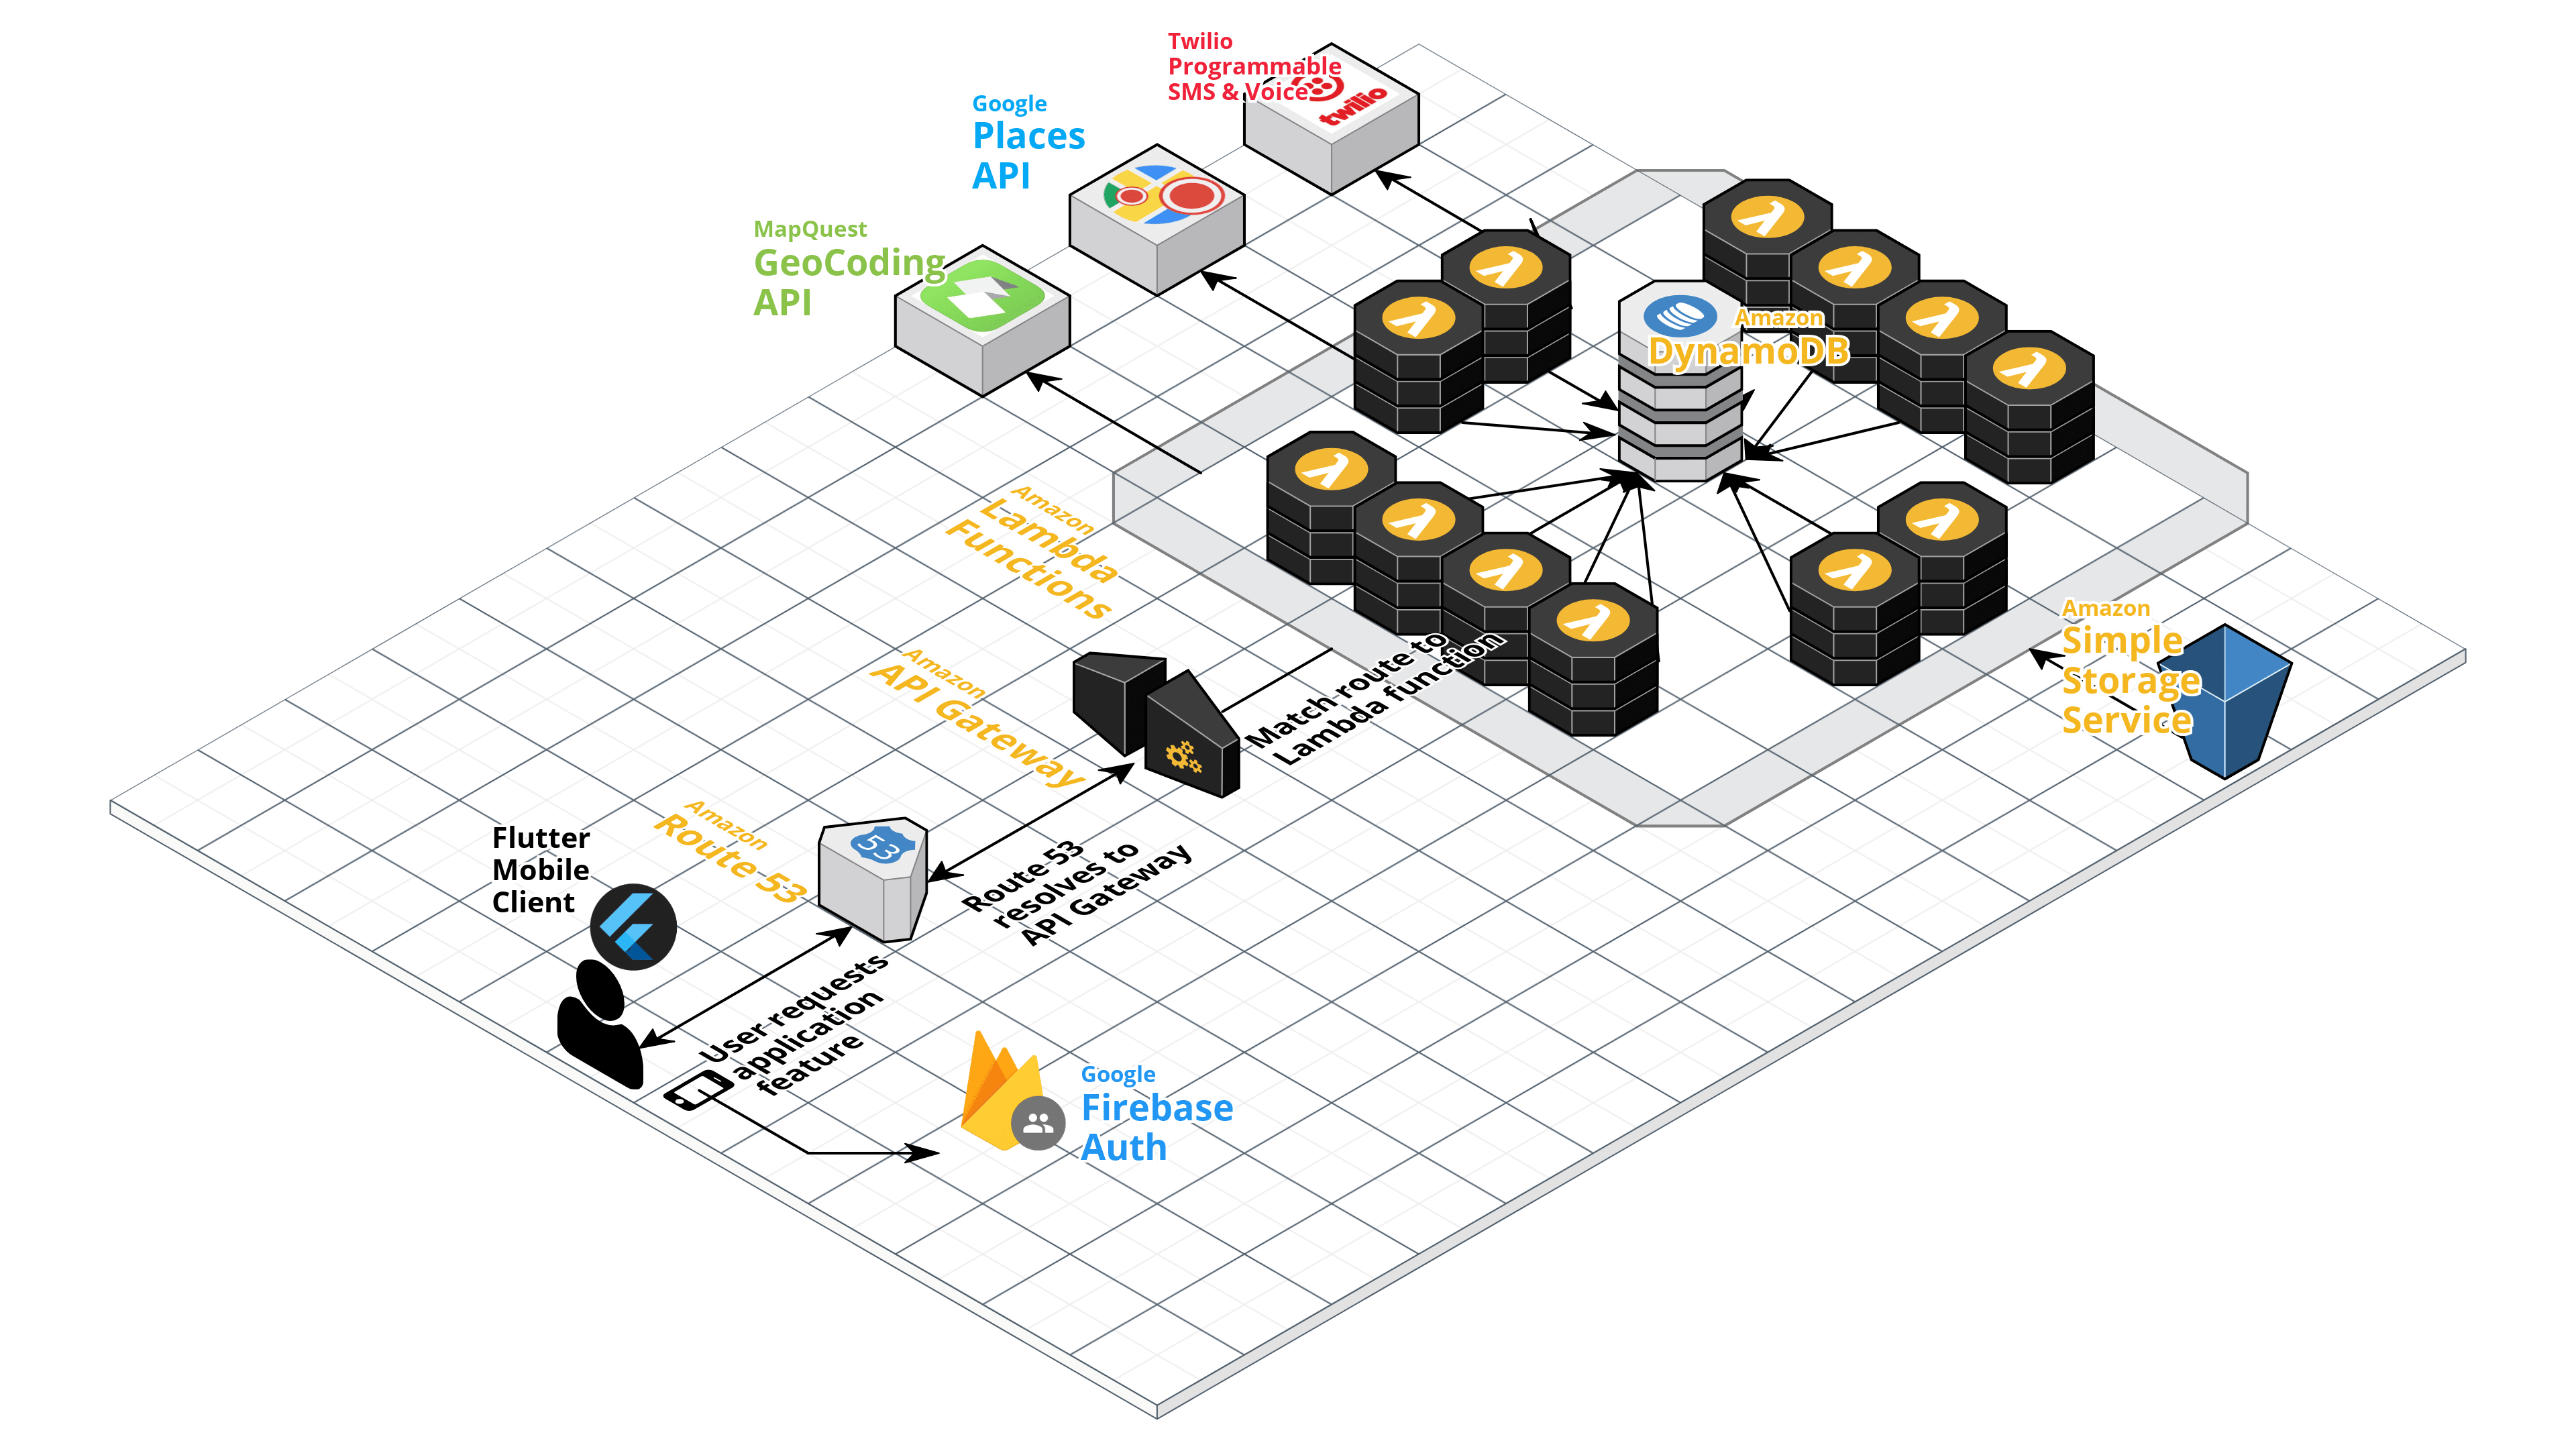
\includegraphics[scale=.2]{EmergenSeek-Backend.PNG}
}
\caption{Updated Cloudcraft diagram of the AWS resources, external APIs encapsulated by the backend, and frontend connection abstractions.}
\end{center}	
\end{figure}

\section{Project Development Lifecycle} 
\label{sec:pdl}
\par ~ Text 

\section{Glossary}
\begin{enumerate}
	\item[$\bullet$] Cross-platform application - software which has a single implementation, but may be executed on different distributions. (i.e. one code base, running on many different operating systems or processor architectures.)
	\item[$\bullet$] Serverless application repository - single responsibility application definitions which act as independent entities. The application repository as a whole defines the API for our mobile application. (i.e. each serverless application is a Lambda function, and the lambda function is responsible for a system feature.)
	\item[$\bullet$] Application Programming Interface (API) - Definitions and communication protocols used for building the structure of software.
	\item[$\bullet$] HyperText Transfer Protocol (HTTP) - An application protocol used heavily for websites and services throughout the Internet.
\end{enumerate}

\begin{thebibliography}{9}
\bibitem{one}
scoped\_model 1.0.1 | Flutter Package --- \url{https://pub.dartlang.org/packages/scoped_model}
\bibitem{two}
What is the AWS Serverless Application Model (AWS SAM)? ~ \url{https://docs.aws.amazon.com/serverless-application-model/latest/developerguide/what-is-sam.html}
\end{thebibliography}

% Appendix of figures
\begin{appendix}
	\listoffigures
\end{appendix}

\end{document}

